\documentclass[11pt]{article}
\usepackage{amsmath, amssymb}
\usepackage{graphicx}
\usepackage{hyperref}
\usepackage{geometry}
\usepackage{fancyhdr}

\pagestyle{fancy}
\fancyhf{}
\fancyfoot[R]{\thepage}
\geometry{margin=1in}

\title{Yet another Trading Strategy (YaTS) on TSX Energy Names}
\date{}

\begin{document}
    \maketitle

    This document lays out a practical trading workflow that connects machine-learning forecasts to clear trading rules. We focus on a small set of liquid Canadian energy names on the Toronto Stock Exchange (think Enbridge and peers), use daily bars, and consider multi-day horizons $n \in \{1,5,20\}$. The aim is simple: trade only when the expected benefit—after costs and risk—justifies it. Because fundamentals from WRDS are central, we respect when information becomes public, we handle dividends and ex-dividend mechanics, and we keep an eye on opportunity cost and Canada’s tax treatment when interpreting results.

    \paragraph{Universe, cadence, and data discipline.}
    We track a tight list of TSX energy stocks and operate on the daily close. Market data come as OHLCV; corporate actions (splits, dividends) are applied so returns reflect what an investor would experience. Fundamentals are pulled from WRDS (e.g., Compustat North America) and timestamped by when a typical investor could reasonably know them (announcement/filing plus a conservative delay). Any feature that isn’t available at decision time is shifted or dropped—no peeking ahead.

    \paragraph{Targets and predictions.}
    Each day $t$, the model ingests a feature vector $X_t$ built from price/volume history, microstructure proxies (e.g., spreads if available, volatility-of-volatility), calendar/regime flags, and lagged fundamentals (profitability, leverage, payout and coverage ratios, cash-flow stability). For each $n \in \{1,5,20\}$, it outputs an expected log return $\mu_n(t)$ and an uncertainty measure $\sigma_n(t)$ (or a few quantiles that imply $\sigma$). We may also compute a probability of an up move $p_{\text{up},n}(t)$ for diagnostics, but the trading logic uses $\mu$ (how much we expect to make) and $\sigma$ (how uncertain that is).

    \paragraph{From forecast to trade decision.}
    A forecast is not a trade. We weigh the signal against costs and uncertainty. For each horizon,
    \[
        U_n(t) \;=\; \lvert \mu_n(t) \rvert \;-\; c(t) \;-\; \kappa\,\sigma_n(t),
    \]
    where $c(t)$ is all-in one-way cost (commission, spread/slippage, and a borrow fee if short), and $\kappa$ is a tunable risk buffer. Taking the absolute value means a strong negative $\mu$ is just as actionable (short) as a strong positive $\mu$ (long). If the best horizon has $U_n(t)\le 0$, we do nothing; otherwise we pick $n^{\ast}=\arg\max_{n} U_n(t)$ and set direction by the sign of $\mu_{n^{\ast}}(t)$.

    \paragraph{Sizing by conviction.}
    Position size should grow with conviction, but never without limits. We use a Sharpe-like ratio and cap it:
    \[
        S_t \;=\; \operatorname{clip}\!\Bigl( \beta \cdot \tfrac{\mu_{n^{\ast}}(t)}{\sigma_{n^{\ast}}(t)} \,;\, -S_{\max},\, S_{\max} \Bigr),
    \]
    where $\beta$ controls aggressiveness and $S_{\max}$ is a hard cap (e.g., $\lvert S\rvert\!=\!1$ for all-in). The operator $\operatorname{clip}(x; a,b)$ means $\min\{\max\{x,a\},\,b\}$. Small signal-to-noise means small $\lvert S_t\rvert$; large signal-to-noise means larger size—but never beyond $S_{\max}$.

    \paragraph{Exit rules and time consistency.}
    We do not hold forever. If nothing else triggers first, a time stop closes the position after $n^{\ast}$ days. To protect capital, a stop-loss exits early if the unrealized loss crosses a volatility-scaled threshold; a take-profit locks gains past a preset level. Exits are defined up front and use the same timestamps and price fields as the entry.

    \paragraph{Costs, dividends, and ex-dividend days.}
    Costs $c(t)$ should at least reflect paying roughly half the bid–ask spread when crossing with marketable orders, plus commission; for thinner names or larger orders, an impact term is sensible. Because dividend payers are central to this universe, we explicitly carry ex-dividend dates: on the ex-date, price typically adjusts down by about the cash dividend, though the exact move depends on ticks, taxes, and market conditions. In backtests we line up dividend cash receipts with ex/record/payable dates and keep corporate-action adjustments consistent so that predicted returns and realized P\&L can be compared fairly.

    \paragraph{Opportunity cost and Canadian tax context.}
    Money in a stock cannot also sit in a cash-like instrument. When comparing choices (including holding through a dividend), we track a cash benchmark to show what was forgone. For a Canadian resident’s after-tax view, two items matter: (i) eligible dividends from taxable Canadian corporations are grossed up and come with dividend tax credits (federal and provincial); (ii) capital gains are taxed via an inclusion rate that can vary by taxpayer type and, above a threshold, by amount or date. We do not bake personal tax into trading P\&L; instead, we can show a side-by-side after-tax lens using current public rules, and call out TFSA/RRSP/RRIF accounts separately because sheltering changes the effective drag.

    \paragraph{Training and evaluation, kept simple.}
    We split history into rolling windows: train on the past, tune on the next slice, test on the following unseen slice. Because labels at different horizons can overlap, we leave a small gap between train and tune so the model doesn’t learn near-duplicates on both sides. Losses match what we predict (e.g., Gaussian negative log-likelihood for $\mu$ and $\sigma$, or pinball loss for quantiles). When choosing a final setting, we look at net test Sharpe with sensible penalties for excessive turnover and deep drawdowns, and we also check calibration to confirm that bigger predicted moves tend to happen more often than smaller ones.

    \paragraph{Reports and traceability.}
    Each run outputs a clear equity curve (gross and net), a trade log with reasons for entries/exits, turnover, hit rate, average trade P\&L, drawdowns, and a cost breakdown (commission, spread/slippage, borrow). For dividend payers we show both price-only and total-return series. A short appendix can add a stylized after-tax view for a Canadian resident—clearly labelled as a simple estimate, not advice. Everything is reproducible from a saved configuration that pins data snapshots, feature recipes, and model versions.

    \paragraph{Diagram.}
    The digram outline the full pipeline from data collection to model training to trading decisions.
    \begin{figure}[h]
        \centering
        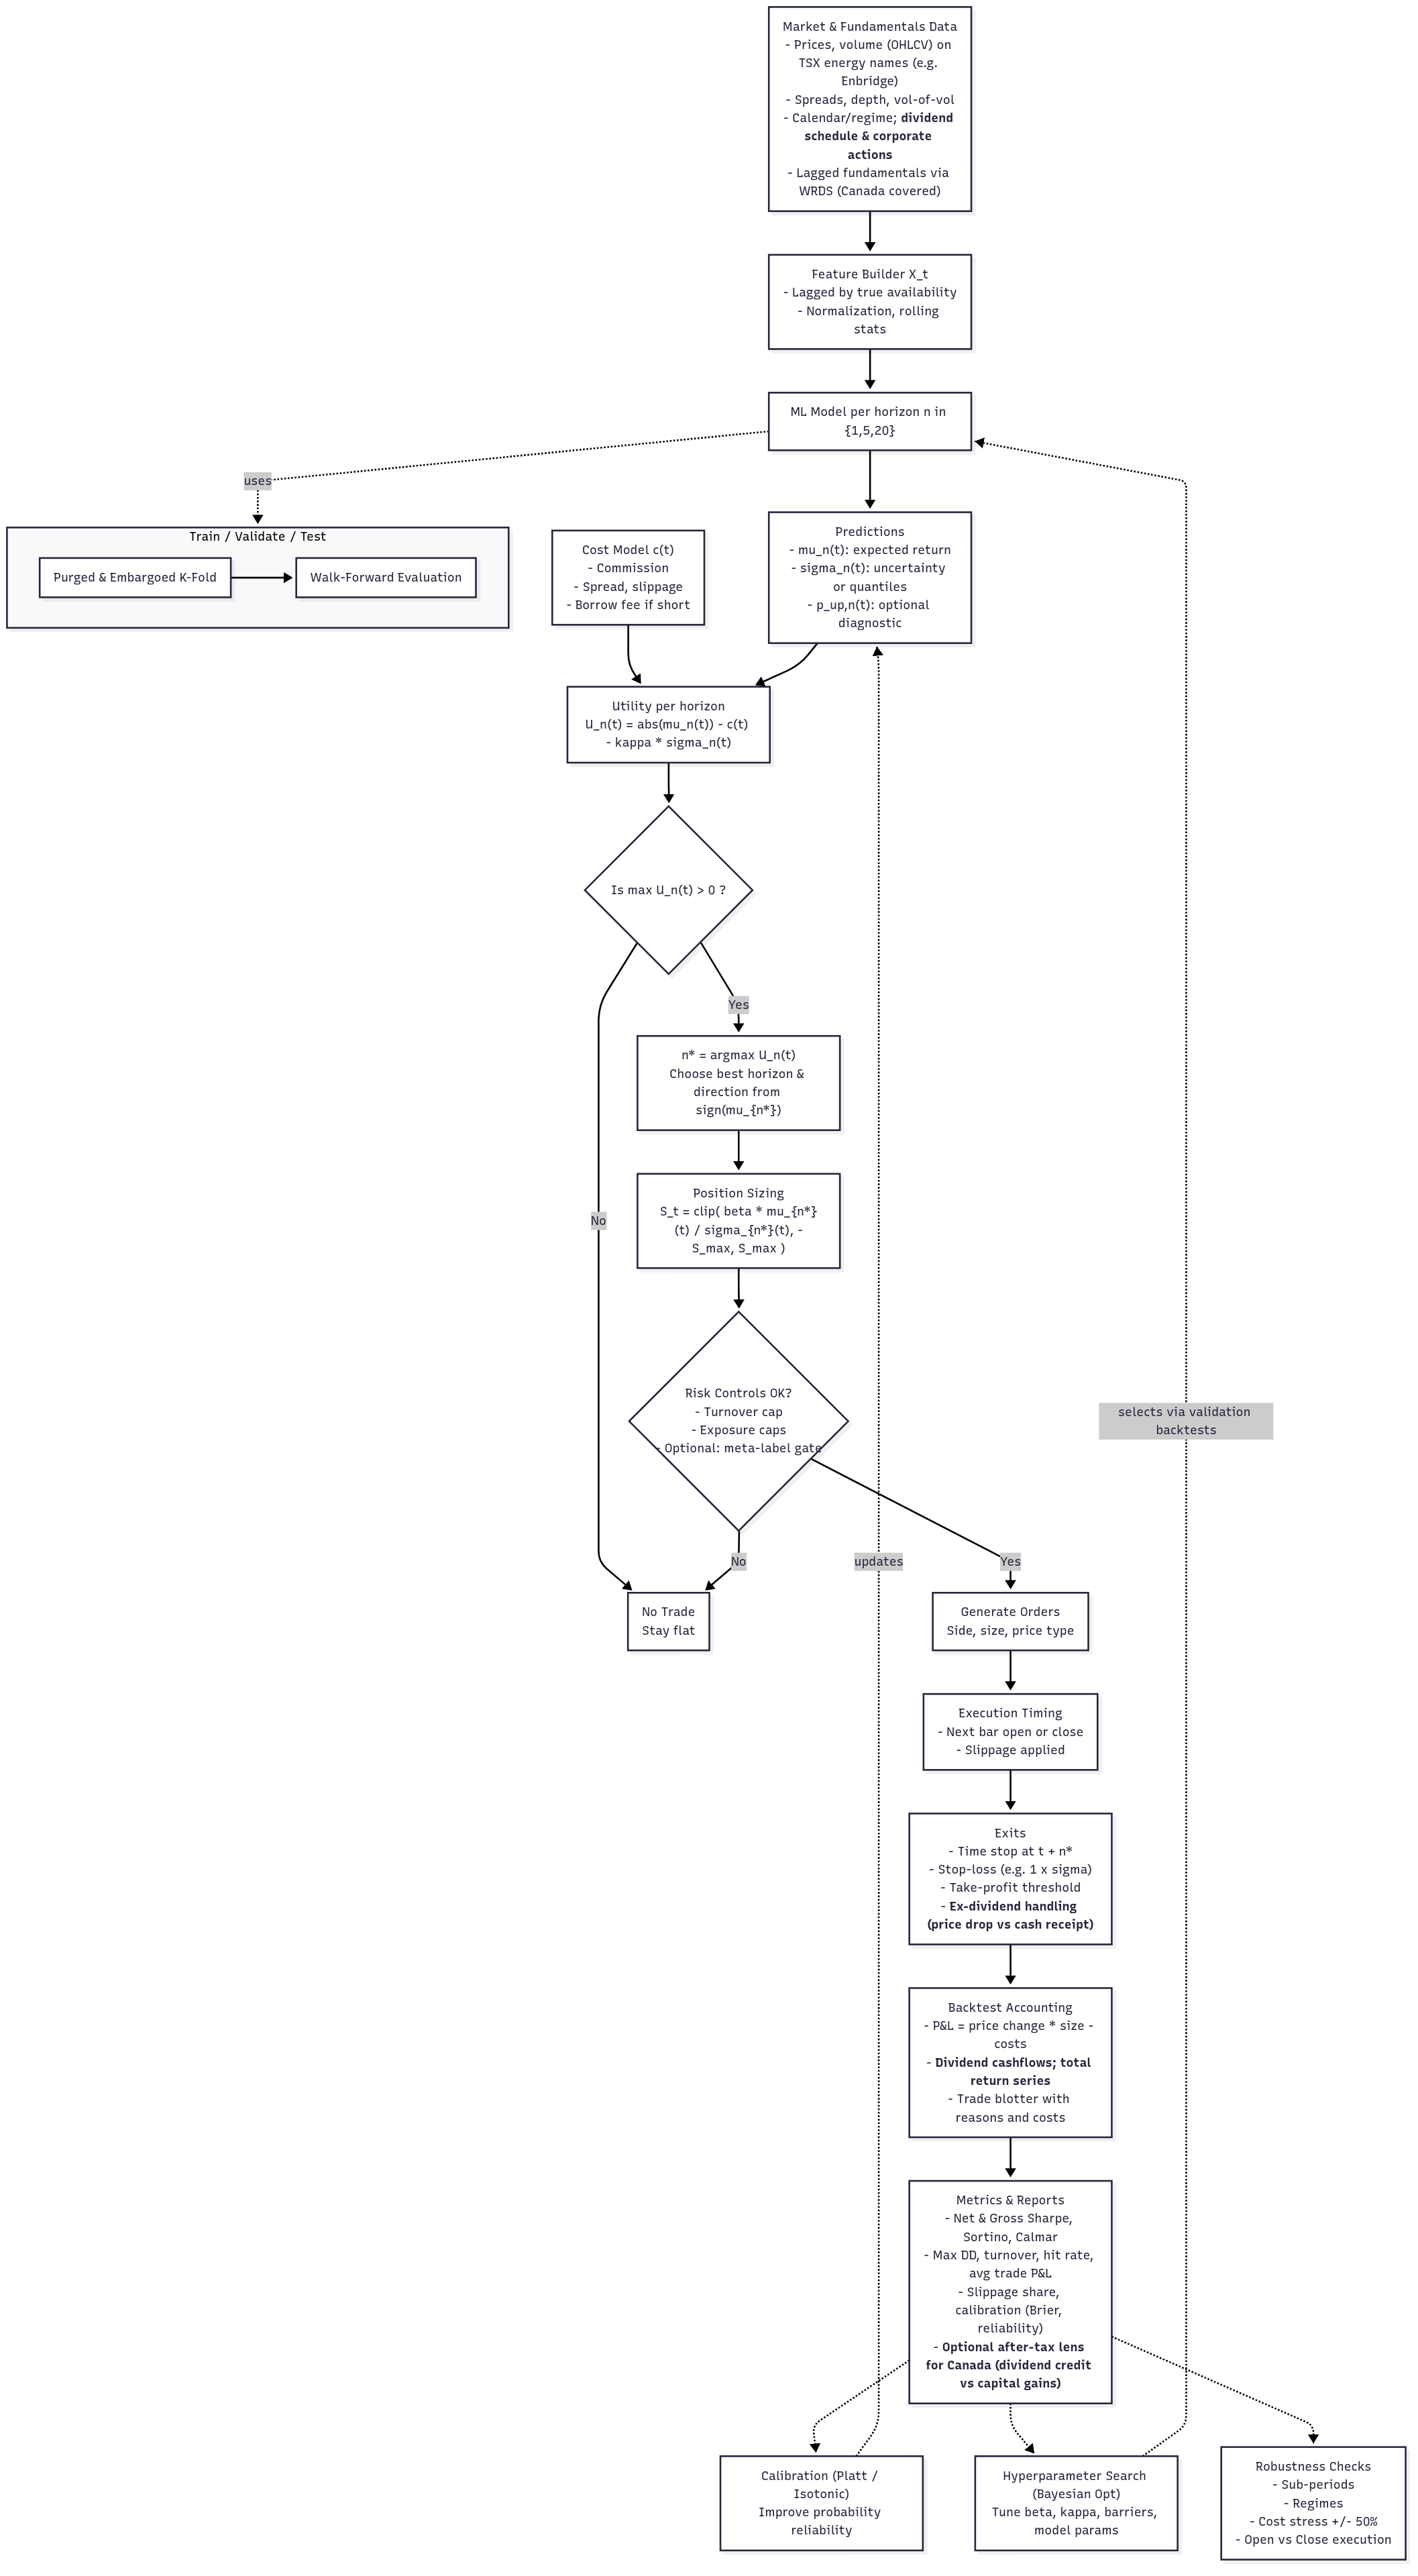
\includegraphics[width=0.78\linewidth,keepaspectratio]{fig/pipeline}
        \caption{Overview from data to reports.}\label{fig:figure}
    \end{figure}

\end{document}